\documentclass[spanish]{beamer}
\usepackage[utf8]{inputenc}
\usepackage{float}
\usepackage{beamerthemesplit}
\usepackage{latexsym}
\usepackage[T1]{fontenc}
\usepackage{amsmath}

\usepackage{hyperref}
\usepackage{graphicx}
\usepackage{babel,blindtext}
\usepackage{amsfonts}
\usepackage[round]{natbib}
\bibliographystyle{chicago}
\usepackage{subcaption} 


\decimalpoint

%\documentclass{beamer}
\usetheme[pageofpages=of,% String used between the current page and the
                         % total page count.
          bullet=circle,% Use circles instead of squares for bullets.
          titleline=true,% Show a line below the frame title.
          alternativetitlepage=true,% Use the fancy title page.
          titlepagelogo=logo,% Logo for the first page.
          watermark=logo2,% Watermark used in every page.
          watermarkheight=60px,% Height of the watermark.
          watermarkheightmult=3,% The watermark image is 4 times bigger
                                % than watermarkheight.
          ]{Torino}

%
%\usetheme{Antibes}%este es el templete que se usa a lo largo de la presentacion
%%themes
%%   default
%%   Boadilla
%%   Madrid
%%   Pittsburgh
%%   Copenhagen
%%   Warsaw
%%   Singapore
%%   Malmoe
%\newcommand\Fontvi{\fontsize{6}{7.2}\selectfont}
\mode<presentation>%tipo de 
\begin{document}

%%%%%%%%%%%%%%%%%%%%%%%%%%%%%%%%%%%%%%%%%%%%%%%%%%%%%%%%%%%%%%%%%%%%%%%%%%%%%%%%%%%%%%%%%%%%%%%%%%%%%%%%%%%%%
\title{Introduction}
\subtitle{Pattern Recognition}
\author{Gamaliel Moreno Chávez}
\institute{MCPI}
\date{Enero-Julio\\ 2021}%para que ponga la fecha de hoy 

\frame{\titlepage}
%%%%%%%%%%%%%%%%%%%%%%%%%%%%%%%%%%%%%%%%%%%%%%%%%%%%%%%%%%%%%%%%%%%%%%%%%%%%%%%%%%%%%%%%%%%%%%%%%%%%%%%%%%%%%
%%%%%%%%%%%%%%%%%%%%%%%%%%%%%%%%%%%%%%%%%%%%%%%%%%%%%%%%%%%%%%%%%%%%%%%%%%%%%%%%%%%%%%%%%%%%%%%%%%%%%%%%%%%%%%%%%%%%%%%%%%%%%%%%%%%%%%%%%%%%%%%%%%%%%%%%%%%%%%%%%%%%%%%%%%%%%%%%%%%%%%%%%%%%%%%%%%%%%%%%%%%%%%%%%%%%%%%%%%
%%%%%%%%%%%%%%%%%%%%%%%%%%%%%%%%%%%%%%%%%%%%%%%%%%%%%%%%%%%%%%%%%%%%%%%%%%%%%%%%%%%%%%%%%%%%%%%%%%%%%%%%%%%%%%%%%%%%%%%%%%%%%%%%%%%%%%%%%%%%%%%%%%%%%%%%%%%%%%%%%%%%%%%%%%%%%%%%%%%%%%%%%%%%%%%%%%%%%%%%%%%%%%%%%%%%%%%%%%

\begin{frame}
\frametitle{Introduction}
IS PATTERN RECOGNITION IMPORTANT?

Pattern recognition is the scientific discipline whose goal is the classification of
objects into a number of categories or classes. We will refer to these objects using the generic term patterns

\begin{itemize}
\item Machine vision
\item Character (letter or number) recognition
\item Computer-aided diagnosis
\item Speech recognition
\end{itemize}


\end{frame}

%%%%%%%%%%%%%%%%%%%%%%%%%%%%%%%%%%%%%%%%%%%%%%%%%%%%%%%%%%%%%%%%%%%%%%%%%%%%%%%%%%%%%%%%%%%%%%%%%%%%%%%%%%%%%
\begin{frame}
\frametitle{Introduction}
What is machine learning?

\begin{block}{Machine Learning or ML}
A computer program is said to learn from experience E with respect to some class of tasks T,
and performance measure P, if its performance at tasks in T, as measured by P, improves with
experience E.
\end{block}
we treat all unknown quantities (e.g., predictions about the future value of some quantity of interest, such as tomorrow’s temperature, or the parameters of some
model) as random variables, that are endowed with probability distributions which describe a weighted set of possible values the variable may have.
\end{frame}
%%%%%%%%%%%%%%%%%%%%%%%%%%%%%%%%%%%%%%%%%%%%%%%%%%%%%%%%%%%%%%%%%%%%%%%%%%%%%%%%%%%%%%%%%%%%%%%%%%%%%%%%%%%%%
\begin{frame}
\frametitle{Introduction}
Probabilistic modeling is the language used by most other areas of science and engineering

\begin{center}
\textit{Almost all of machine learning can be viewed in probabilistic terms, making probabilistic
thinking fundamental. It is, of course, not the only view. But it is through this view that we
can connect what we do in machine learning to every other computational science, whether that
be in stochastic optimization, control theory, operations research, econometrics, information
theory, statistical physics or bio-statistics. For this reason alone, mastery of probabilistic
thinking is essential.}
\end{center}
\end{frame}
%%%%%%%%%%%%%%%%%%%%%%%%%%%%%%%%%%%%%%%%%%%%%%%%%%%%%%%%%%%%%%%%%%%%%%%%%%%%%%%%%%%%%%%%%%%%%%%%%%%%%%%%%%%%%
\begin{frame}
\frametitle{Introduction}
Learning types: Supervised and Unsupervised learning
\begin{center}
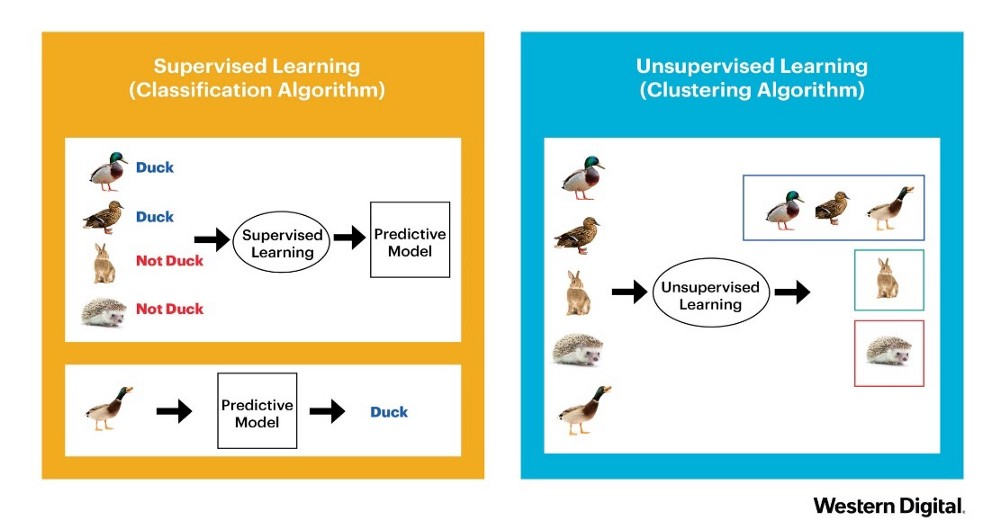
\includegraphics[scale=0.35]{im1}
\end{center}


\end{frame}
%%%%%%%%%%%%%%%%%%%%%%%%%%%%%%%%%%%%%%%%%%%%%%%%%%%%%%%%%%%%%%%%%%%%%%%%%%%%%%%%%%%%%%%%%%%%%%%%%%%%%%%%%%%%%
\begin{frame}
\frametitle{Introduction}
\textbf{Supervised learning}
\begin{itemize}
\item the task T is to learn a mapping $f$ from inputs $x \in X$ to outputs $y \in Y$.
\item The inputs x are also called the features, covariates, or predictors. This is often a fixed dimensional vector of numbers, such as the height
and weight of a person, or the pixels in an image.
\item $X = \mathbb{R}^{D}$, where $D$ is the dimensionality of the vector.
\item  The output $y$ is also known as the label, target, or response.
\item The experience $E$ is given in the form of a set of $N$ input-output pairs $ \mathcal{D} = \lbrace{(xn, yn)}\rbrace_{n=1}^{N}$ known as the training set.
\item $N$ is called the sample size.
\end{itemize} 

\end{frame}

%%%%%%%%%%%%%%%%%%%%%%%%%%%%%%%%%%%%%%%%%%%%%%%%%%%%%%%%%%%%%%%%%%%%%%%%%%%%%%%%%%%%%%%%%%%%%%%%%%%%%%%%%%%%%
\begin{frame}
\frametitle{Classification} 
In classification problems, the output space is a set of $C$ unordered and mutually exclusive labels
known as classes, $Y = \lbrace1, 2, \ldots ,C\rbrace$. The problem of predicting the class label given an input is
also called pattern recognition. If there are just two classes, often denoted by $y  \in \lbrace 0, 1\rbrace$ or
$y  \in \lbrace 0, 1\rbrace$, it is called binary classification.

\end{frame}
%%%%%%%%%%%%%%%%%%%%%%%%%%%%%%%%%%%%%%%%%%%%%%%%%%%%%%%%%%%%%%%%%%%%%%%%%%%%%%%%%%%%%%%%%%%%%%%%%%%%%%%%%%%%%
\begin{frame}
\frametitle{Classification}  
Example: classifying Iris flowers. Consider the problem of classifying iris flowers into their 3 subspecies, setosa, versicolor
and virginica.
\begin{center}
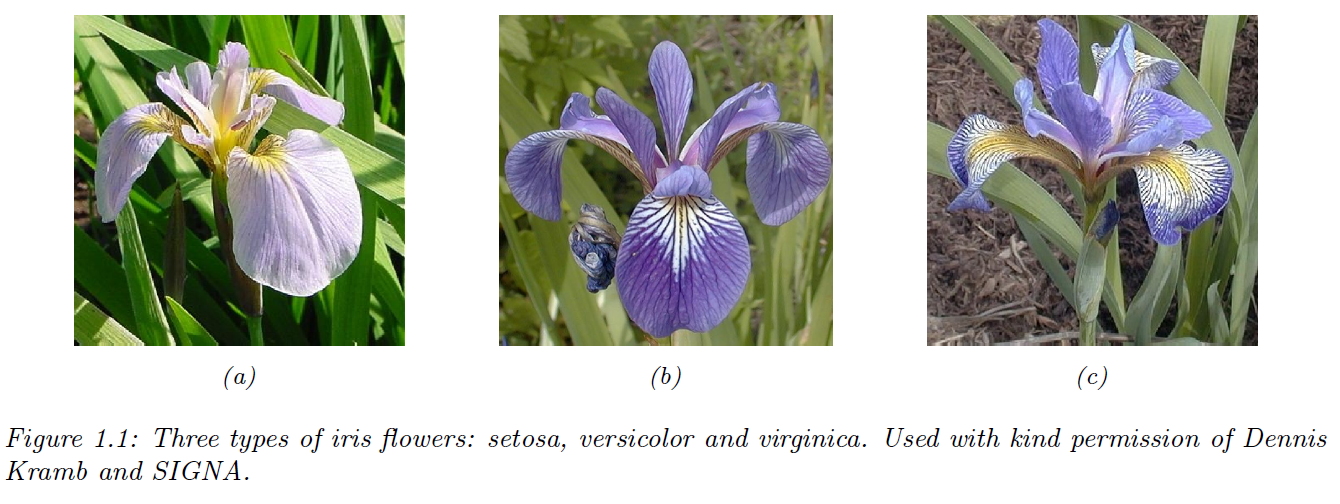
\includegraphics[width=\textwidth]{im2}
\end{center}
\end{frame}
%%%%%%%%%%%%%%%%%%%%%%%%%%%%%%%%%%%%%%%%%%%%%%%%%%%%%%%%%%%%%%%%%%%%%%%%%%%%%%%%%%%%%%%%%%%%%%%%%%%%%%%%%%%%%
\begin{frame}
\frametitle{Classification}  
Example: classifying Iris flowers. Consider the problem of classifying iris flowers into their 3 subspecies, setosa, versicolor
and virginica.
\begin{center}
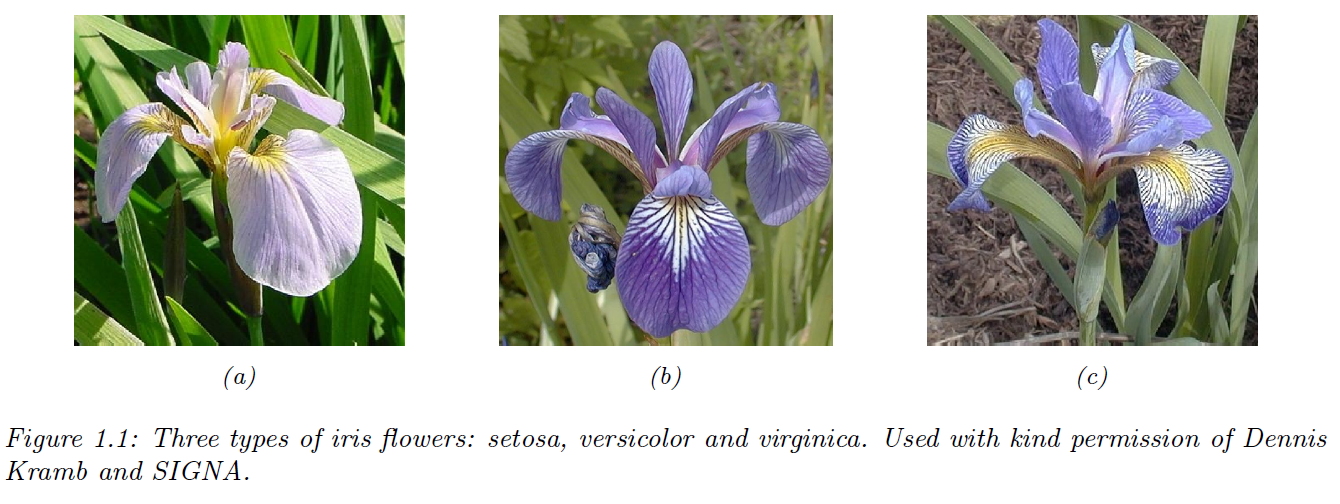
\includegraphics[width=\textwidth]{im2}
\end{center}
\end{frame}
%%%%%%%%%%%%%%%%%%%%%%%%%%%%%%%%%%%%%%%%%%%%%%%%%%%%%%%%%%%%%%%%%%%%%%%%%%%%%%%%%%%%%%%%%%%%%%%%%%%%%%%%%%%%%
\begin{frame}
\frametitle{Classification}  
In image classification, the input space $X$ is the set of images, which is a very high dimensional
space: for a color image with $C = 3$ channels (e.g., RGB) and $D_1 \times  D_2$ pixels, we have $X = \mathbb{R}^{D}$, where $D= C \times D_1 \times D_2$.

Some botanists have already identified 4 simple, but highly informative, numeric
feature: sepal length, sepal width, petal length, petal width

We will use this much lower dimensional input space,$X = \mathbb{R}^{D}$, for simplicity. The iris dataset is a collection of 150 labeled examples of iris flowers, 50 of
each type, described by these 4 features.
\end{frame}
%%%%%%%%%%%%%%%%%%%%%%%%%%%%%%%%%%%%%%%%%%%%%%%%%%%%%%%%%%%%%%%%%%%%%%%%%%%%%%%%%%%%%%%%%%%%%%%%%%%%%%%%%%%%%
\begin{frame}
\frametitle{Classification}  
It is common to store them in an $N\times D$ matrix, in which each row represents an example, and each column represents a feature. This is known as a design
matrix;
\begin{center}
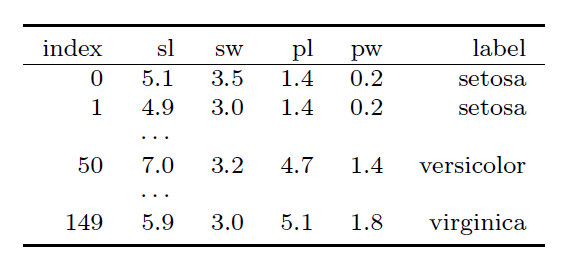
\includegraphics[width=\textwidth]{im3}
\end{center}

\end{frame}
%%%%%%%%%%%%%%%%%%%%%%%%%%%%%%%%%%%%%%%%%%%%%%%%%%%%%%%%%%%%%%%%%%%%%%%%%%%%%%%%%%%%%%%%%%%%%%%%%%%%%%%%%%%%%
\begin{frame}
\frametitle{Classification}  
Exploratory data analysis. Before tackling a problem with ML, it is usually a good idea to perform exploratory data analysis.

\begin{center}
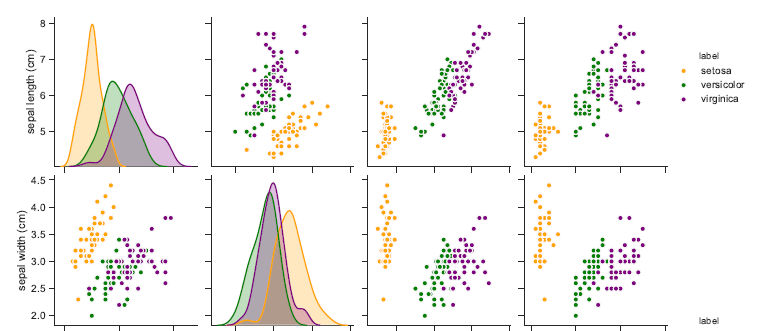
\includegraphics[width=\textwidth]{im4}
\end{center}

\end{frame}
%%%%%%%%%%%%%%%%%%%%%%%%%%%%%%%%%%%%%%%%%%%%%%%%%%%%%%%%%%%%%%%%%%%%%%%%%%%%%%%%%%%%%%%%%%%%%%%%%%%%%%%%%%%%%
\begin{frame}
\frametitle{Classification}  
Exploratory data analysis. Before tackling a problem with ML, it is usually a good idea to perform exploratory data analysis.

\begin{center}
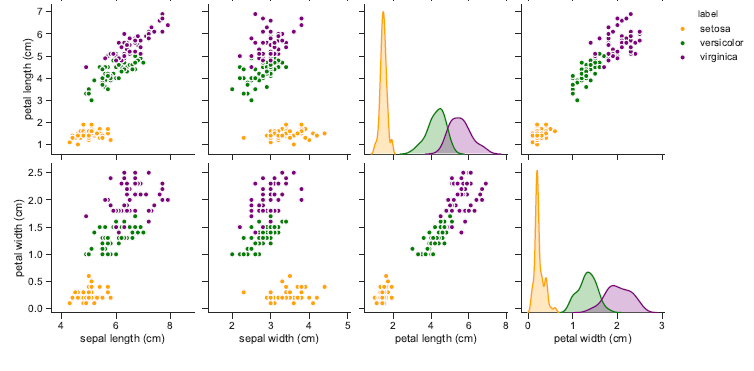
\includegraphics[width=\textwidth]{im5}
\end{center}

\end{frame}
%%%%%%%%%%%%%%%%%%%%%%%%%%%%%%%%%%%%%%%%%%%%%%%%%%%%%%%%%%%%%%%%%%%%%%%%%%%%%%%%%%%%%%%%%%%%%%%%%%%%%%%%%%%%%
\begin{frame}
\frametitle{Classification}  
We can see that the setosa class is easy to distinguish from the other two classes. For
example, suppose we create the following decision rule:

\begin{center}
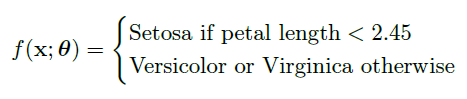
\includegraphics[width=\textwidth]{im6}
\end{center}
\end{frame}
%%%%%%%%%%%%%%%%%%%%%%%%%%%%%%%%%%%%%%%%%%%%%%%%%%%%%%%%%%%%%%%%%%%%%%%%%%%%%%%%%%%%%%%%%%%%%%%%%%%%%%%%%%%%%
\begin{frame}
\frametitle{Classification}  
We can arrange these nested rules in to a tree structure, \textbf{called a decision tree}.
\begin{center}
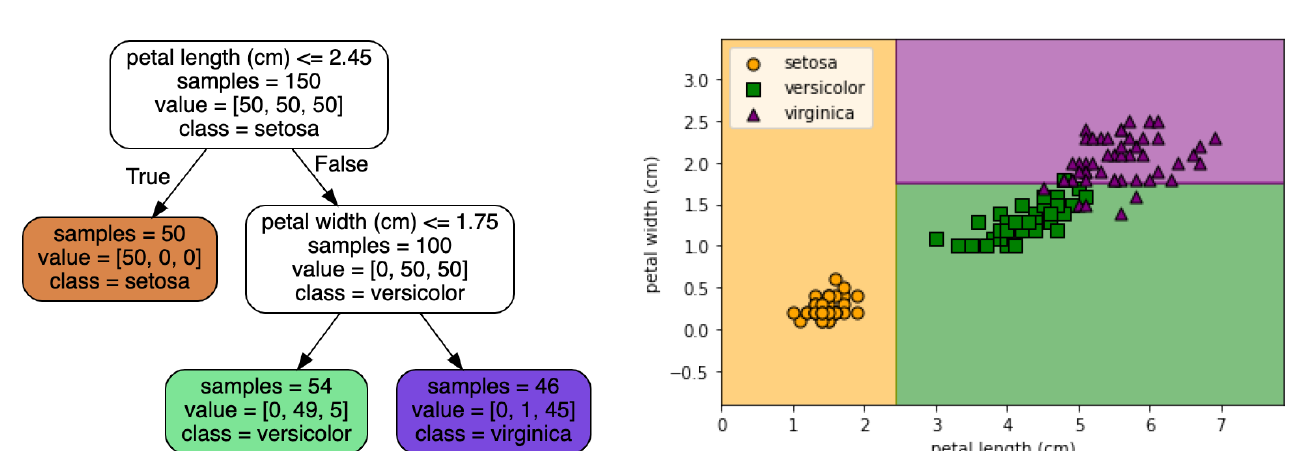
\includegraphics[width=\textwidth]{im7}
\end{center}
\end{frame}
%%%%%%%%%%%%%%%%%%%%%%%%%%%%%%%%%%%%%%%%%%%%%%%%%%%%%%%%%%%%%%%%%%%%%%%%%%%%%%%%%%%%%%%%%%%%%%%%%%%%%%%%%%%%%
\begin{frame}
\frametitle{Model fitting}
The goal of supervised learning is to automatically come up with classification models. A common way to
measure performance on this task is in terms of the misclassification rate on the training set:
\begin{equation*}
\mathcal{L}(\mathbf{\theta}) \triangleq \frac{1}{N} \sum_{n=1}^{N}{\mathbb{I}(y_{n}\neq f(x_{n};\mathbf{\theta})) }
\end{equation*}
where $\mathbb{I}(e)$ is the binary indicator function,
\begin{center}
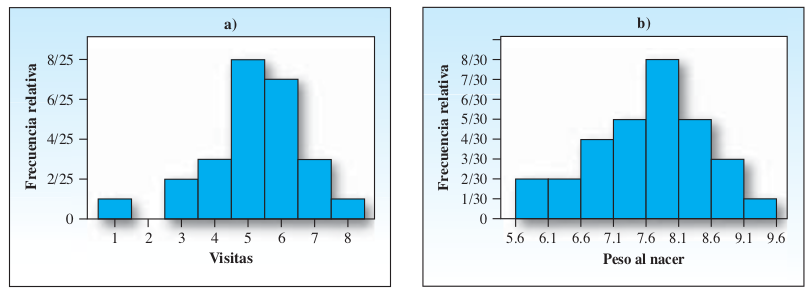
\includegraphics[scale=0.5]{im8}
\end{center}
\end{frame}
%%%%%%%%%%%%%%%%%%%%%%%%%%%%%%%%%%%%%%%%%%%%%%%%%%%%%%%%%%%%%%%%%%%%%%%%%%%%%%%%%%%%%%%%%%%%%%%%%%%%%%%%%%%%%
\begin{frame}
\frametitle{Model fitting}
For example, suppose we are foraging in the wilderness and we find some iris flowers.
Furthermore, suppose that setosa and versicolor are tasty, but virginica is poisonous. In this case, we
might use the asymmetric loss function
\begin{center}
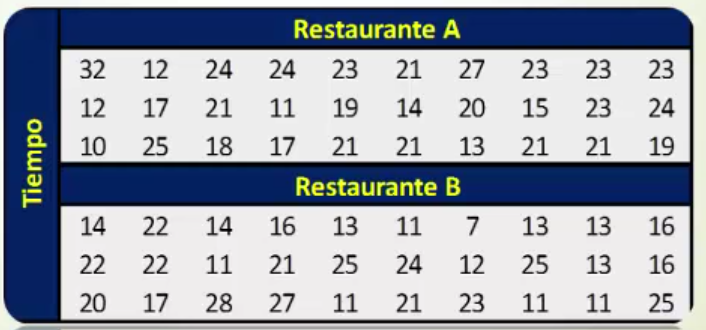
\includegraphics[scale=0.4]{im9}
\end{center}
\end{frame}
%%%%%%%%%%%%%%%%%%%%%%%%%%%%%%%%%%%%%%%%%%%%%%%%%%%%%%%%%%%%%%%%%%%%%%%%%%%%%%%%%%%%%%%%%%%%%%%%%%%%%%%%%%%%%
\begin{frame}
\frametitle{Model fitting}
We can then define empirical risk to be the average loss of the predictor on the training set:
\begin{equation*}
\mathcal{L}(\mathbf{\theta}) \triangleq \frac{1}{N} \sum_{n=1}^{N}{\mathscr{l}(y_{n}, f(x_{n};\mathbf{\theta})) }
\end{equation*}
the empirical risk is equal to misclassification rate when we use zero-one loss for comparing the true label with the prediction
\begin{equation*}
\textit{l}_{01}(y,\hat{y})= \mathbb{I}(y_{n}\neq \hat{y}) 
\end{equation*} 

\end{frame}
%%%%%%%%%%%%%%%%%%%%%%%%%%%%%%%%%%%%%%%%%%%%%%%%%%%%%%%%%%%%%%%%%%%%%%%%%%%%%%%%%%%%%%%%%%%%%%%%%%%%%%%%%%%%%
\begin{frame}
\frametitle{Model fitting}
One way to define the problem of model fitting or training is to find a setting of the parameters
that minimizes the empirical risk on the training set:
\begin{equation*}
\hat{\theta} =  \arg\min_{\theta} \mathcal{L}(\mathbf{\theta})  =\arg\min_{\theta} \frac{1}{N} \sum_{n=1}^{N}{l(y_{n}, f(x_{n};\mathbf{\theta})) }
\end{equation*}
This is called empirical risk minimization.
\end{frame}

%%%%%%%%%%%%%%%%%%%%%%%%%%%%%%%%%%%%%%%%%%%%%%%%%%%%%%%%%%%%%%%%%%%%%%%%%%%%%%%%%%%%%%%%%%%%%%%%%%%%%%%%%%%%%
\begin{frame}
\frametitle{Rango}
\begin{block}{Definición}
El rango, R, de un conjunto de n mediciones se define como la diferencia entre la medición más grande y la más pequeña.
\end{block}
\vspace{1em}

Para los datos de peso al nacer de la tabla, las mediciones varían de 5.6 a 9.4. Por tanto, el rango es $9.4-5.6 =3.8$.
\begin{center}
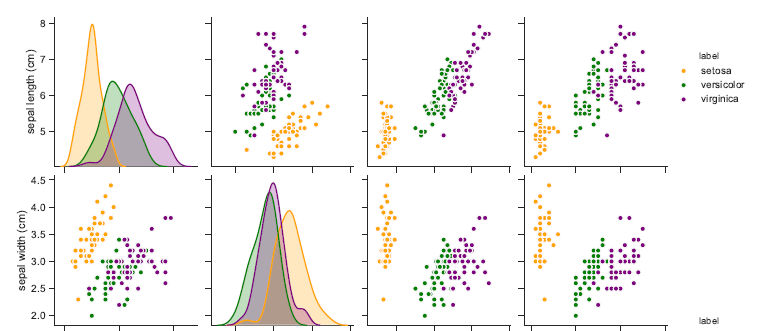
\includegraphics[scale=0.5]{im4}
\end{center}
\end{frame}

%%%%%%%%%%%%%%%%%%%%%%%%%%%%%%%%%%%%%%%%%%%%%%%%%%%%%%%%%%%%%%%%%%%%%%%%%%%%%%%%%%%%%%%%%%%%%%%%%%%%%%%%%%%%%
\begin{frame}
\frametitle{Rango}
El rango es fácil de calcular, fácil de interpretar
y es una medida adecuada de variación para conjuntos pequeños de datos. Pero, para conjuntos grandes, el rango no es una medida adecuada de variabilidad. Por ejemplo, las dos distribuciones de frecuencia relativa de la figura tienen el mismo rango pero muy diferentes formas y variabilidad.
\begin{center}
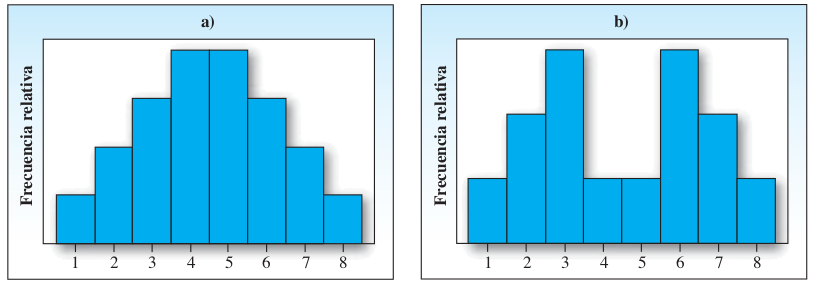
\includegraphics[width=\textwidth]{im12}
\end{center}
\end{frame}


%%%%%%%%%%%%%%%%%%%%%%%%%%%%%%%%%%%%%%%%%%%%%%%%%%%%%%%%%%%%%%%%%%%%%%%%%%%%%%%%%%%%%%%%%%%%%%%%%%%%%%%%%%%%%
\begin{frame}
\frametitle{Varianza}
¿Hay una medida de variabilidad que sea más sensible que el rango?
\begin{columns}
\column{0.6\textwidth}
\begin{center}
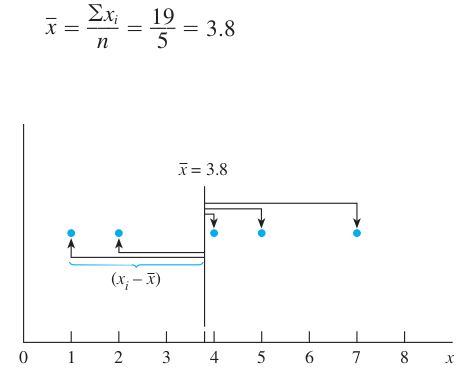
\includegraphics[width=\textwidth]{im13}
\end{center}

\column{0.4\textwidth}
\begin{center}
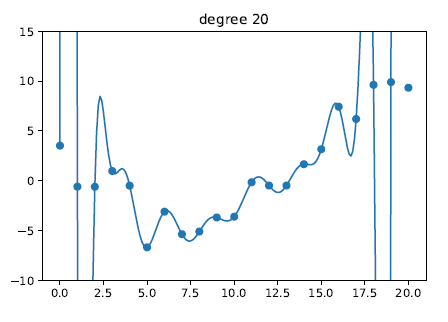
\includegraphics[width=\textwidth]{im14}
\end{center}
\end{columns}

\end{frame}
%%%%%%%%%%%%%%%%%%%%%%%%%%%%%%%%%%%%%%%%%%%%%%%%%%%%%%%%%%%%%%%%%%%%%%%%%%%%%%%%%%%%%%%%%%%%%%%%%%%%%%%%%%%%%
\begin{frame}
\frametitle{Varianza}
De la suma de desviaciones cuadradas, se calcula una sola medida llamada varianza. Para la varianza de una muestra usamos el símbolo $s^2$ y la varianza de una población $\sigma^2$. La varianza será relativamente grande para datos muy variables y relativamente pequeña para datos menos variables.
\begin{block}{Definición}
La \textbf{varianza de una población} de $N$ mediciones es el promedio de los
cuadrados de las desviaciones de las mediciones alrededor de su media $\mu$. La varianza poblacional se denota con $\sigma^2$ y está dada por la fórmula
\begin{equation*}
\sigma^2= \frac{\sum {(x_{i}- \mu)}^2}{N}
\end{equation*}
\end{block}

\end{frame}
%%%%%%%%%%%%%%%%%%%%%%%%%%%%%%%%%%%%%%%%%%%%%%%%%%%%%%%%%%%%%%%%%%%%%%%%%%%%%%%%%%%%%%%%%%%%%%%%%%%%%%%%%%%%%
\begin{frame}
\frametitle{Varianza}

\begin{block}{Definición}
La \textbf{varianza de una muestra} de $n$ mediciones es la suma de las desviaciones cuadradas de las mediciones alrededor la media $\bar{x}$ dividida entre $(n-1)$. La varianza muestral se denota con $s^2$ y está dada por la fórmula 

\begin{equation*}
s^2= \frac{\sum {(x_{i}- \bar{x})}^2}{n-1}
\end{equation*}
\end{block}

\end{frame}
%%%%%%%%%%%%%%%%%%%%%%%%%%%%%%%%%%%%%%%%%%%%%%%%%%%%%%%%%%%%%%%%%%%%%%%%%%%%%%%%%%%%%%%%%%%%%%%%%%%%%%%%%%%%%
\begin{frame}
\frametitle{Varianza}
Para el conjunto de $n = 5$ mediciones muestrales presentadas en la tabla
\begin{columns}
\column{0.6\textwidth}
suma
\begin{equation*}
\sum {(x_{i}- \bar{x})}^2=22.80
\end{equation*}
varianza muestral

\begin{equation*}
s^2= \frac{\sum {(x_{i}- \bar{x})}^2}{n-1}= \frac{22.80}{4}=5.70
\end{equation*}

\column{0.4\textwidth}
\begin{center}
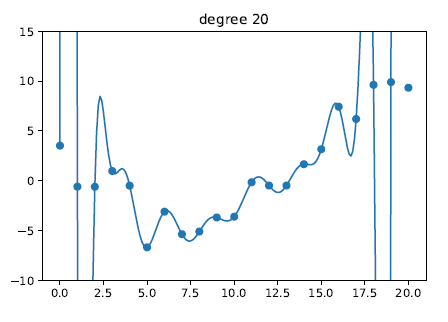
\includegraphics[width=\textwidth]{im14}
\end{center}
\end{columns}

\end{frame}
%%%%%%%%%%%%%%%%%%%%%%%%%%%%%%%%%%%%%%%%%%%%%%%%%%%%%%%%%%%%%%%%%%%%%%%%%%%%%%%%%%%%%%%%%%%%%%%%%%%%%%%%%%%%%
\begin{frame}
\frametitle{Desviación estándar}
La varianza se mide en términos del cuadrado de las unidades originales de medición. Tomando la raíz cuadrada de la varianza, obtenemos la desviación estándar, que regresa la medida de variabilidad a las unidades originales de medición.

\begin{block}{Definición}
La \textbf{desviación estándar} de un conjunto de mediciones es igual a la raíz
cuadrada positiva de la varianza.
\end{block}
\end{frame}
%%%%%%%%%%%%%%%%%%%%%%%%%%%%%%%%%%%%%%%%%%%%%%%%%%%%%%%%%%%%%%%%%%%%%%%%%%%%%%%%%%%%%%%%%%%%%%%%%%%%%%%%%%%%%
\begin{frame}
\frametitle{Notación}

\begin{center}
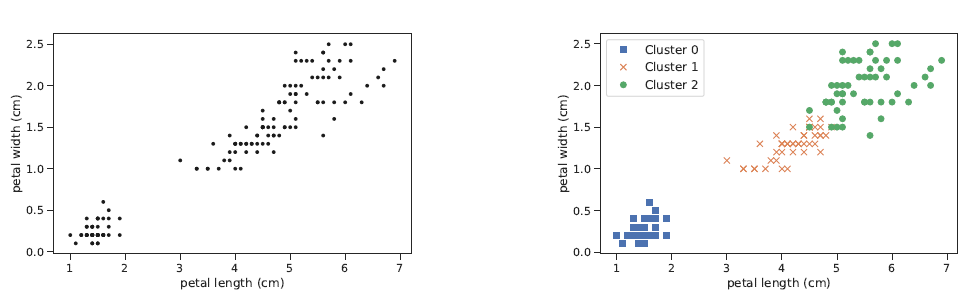
\includegraphics[width=\textwidth]{im15}
\end{center}

\end{frame}
%%%%%%%%%%%%%%%%%%%%%%%%%%%%%%%%%%%%%%%%%%%%%%%%%%%%%%%%%%%%%%%%%%%%%%%%%%%%%%%%%%%%%%%%%%%%%%%%%%%%%%%%%%%%%
\begin{frame}
\frametitle{Resumen}

\begin{center}
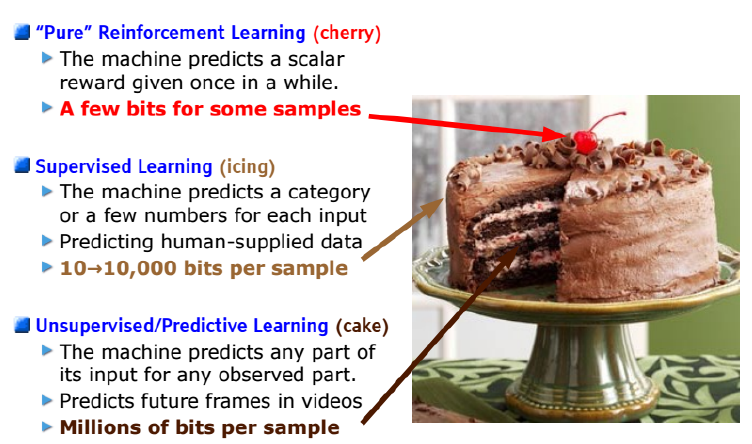
\includegraphics[width=\textwidth]{im16}
\end{center}

\end{frame}
%%%%%%%%%%%%%%%%%%%%%%%%%%%%%%%%%%%%%%%%%%%%%%%%%%%%%%%%%%%%%%%%%%%%%%%%%%%%%%%%%%%%%%%%%%%%%%%%%%%%%%%%%%%%%
\begin{frame}
\frametitle{Coeficiente de variación}
El coeficiente de variación es la relación entre la desviación típica de una muestra y su media.
\begin{equation*}
CV=\left( \frac{\sigma}{\bar{x}} \right) 100
\end{equation*}
El coeficiente de variación permite comparar las dispersiones de dos distribuciones distintas, siempre que sus medias sean positivas.

Mayor dispersión el valor del coeficiente de variación será mayor.
\end{frame}
%%%%%%%%%%%%%%%%%%%%%%%%%%%%%%%%%%%%%%%%%%%%%%%%%%%%%%%%%%%%%%%%%%%%%%%%%%%%%%%%%%%%%%%%%%%%%%%%%%%%%%%%%%%%%
\begin{frame}
\frametitle{Coeficiente de variación}
Una distribución tiene $\bar{x}=140$ y $\sigma =28.28$ y otra $\bar{x}=150$ y $\sigma =24$. ¿Cuál de las dos presenta mayor dispersión?

\begin{equation*}
\textup{CV}_{1}=\cfrac{28,28}{140}\cdot 100=20,2 \%
\end{equation*}
 
\begin{equation*}
\textup{CV}_{2}=\cfrac{24}{150}\cdot 100=16 \%
\end{equation*}
 
La primera distribución presenta mayor dispersión.

\end{frame}
%%%%%%%%%%%%%%%%%%%%%%%%%%%%%%%%%%%%%%%%%%%%%%%%%%%%%%%%%%%%%%%%%%%%%%%%%%%%%%%%%%%%%%%%%%%%%%%%%%%%%%%%%%%%%
\begin{frame}
\frametitle{Sobre la significancia práctica de la desviación estándar}

\begin{block}{Teorema de Chebyshev}
Dado un número $k$ mayor o igual a $1$ y un conjunto de n mediciones, al menos $[1 - (1/k^2)]$ de las mediciones estarán dentro de $k$ desviaciones estándar de su media.
\end{block}

Se construye un intervalo al medir una distancia $k\sigma$ a cualquier lado de la media $m$. El número $k$ puede ser cualquier número mientras sea mayor o igual a 1. Entonces el teorema de Chebyshev expresa que al menos $[1 - (1/k^2)]$ del número total $n$ de mediciones está en el intervalo construido.

\end{frame}
%%%%%%%%%%%%%%%%%%%%%%%%%%%%%%%%%%%%%%%%%%%%%%%%%%%%%%%%%%%%%%%%%%%%%%%%%%%%%%%%%%%%%%%%%%%%%%%%%%%%%%%%%%%%%
\begin{frame}
\frametitle{Teorema de Chebyshev}
Ilustración del teorema de Chebyshev
\begin{center}
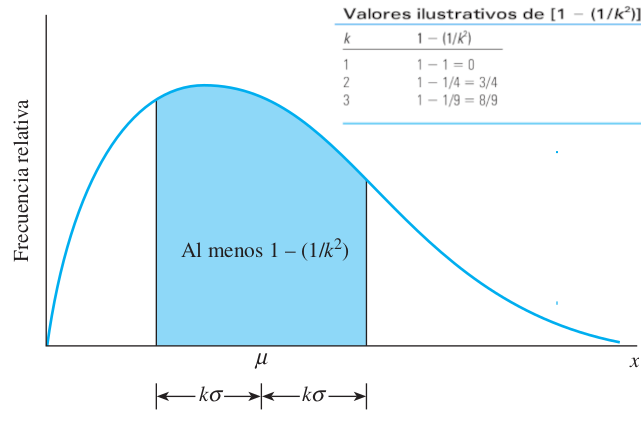
\includegraphics[width=0.8\textwidth]{im17}
\end{center}


\end{frame}
%%%%%%%%%%%%%%%%%%%%%%%%%%%%%%%%%%%%%%%%%%%%%%%%%%%%%%%%%%%%%%%%%%%%%%%%%%%%%%%%%%%%%%%%%%%%%%%%%%%%%%%%%%%%%
\begin{frame}
\frametitle{Teorema de Chebyshev}
Ilustración del teorema de Chebyshev
\begin{center}
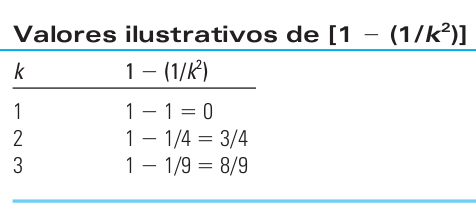
\includegraphics[scale=0.4]{im18}
\end{center}
\begin{center}
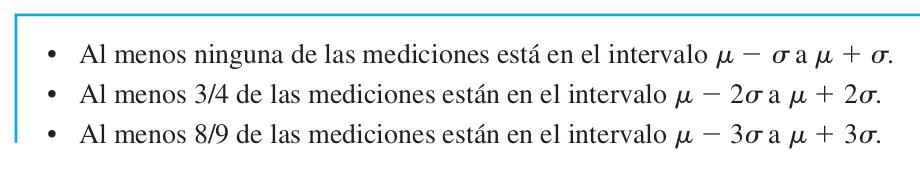
\includegraphics[width=\textwidth]{im19}
\end{center}

\end{frame}
%%%%%%%%%%%%%%%%%%%%%%%%%%%%%%%%%%%%%%%%%%%%%%%%%%%%%%%%%%%%%%%%%%%%%%%%%%%%%%%%%%%%%%%%%%%%%%%%%%%%%%%%%%%%%
\begin{frame}
\frametitle{Teorema de Chebyshev}
Ejemplo. La media y varianza de una muestra de $n = 25$ mediciones son $75$ y $100$, respectivamente. Use el teorema de Chebyshev para describir la distribución de mediciones.

Solución Nos dan $\bar{x} =75$ y $s^2 = 100$. La desviación estándar es $s =\sqrt{100}=10$. La distribución de mediciones está centrada alrededor de x = 75, y el teorema de Chebyshev establece que:
\begin{itemize}
\item Al menos $3/4$ de las 25 mediciones están en el intervalo $\bar{x} \pm  2s = 75 \pm 2(10)$, esto es, $55$ a $95$.

\item Al menos $8/9$ de las mediciones están en el intervalo $\bar{x} \pm  3s = 75 \pm 3(10)$, esto es, 45 a 105.
\end{itemize}


\end{frame}
%%%%%%%%%%%%%%%%%%%%%%%%%%%%%%%%%%%%%%%%%%%%%%%%%%%%%%%%%%%%%%%%%%%%%%%%%%%%%%%%%%%%%%%%%%%%%%%%%%%%%%%%%%%%%
\begin{frame}
\frametitle{Regla empírica}
Como el teorema de Chebyshev se aplica a cualquier distribución, es muy conservador. Ésta es la razón por la que hacemos hincapié en “al menos $1 - (1/k ^2)$” en este teorema. Otra regla para describir la variabilidad de un conjunto de datos no funciona para todos los conjuntos de datos, pero funciona muy bien para datos que “se apilan” en la conocida forma de montículo de la figura

\begin{center}
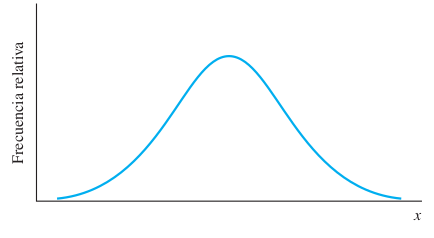
\includegraphics[scale=0.4]{im20}
\end{center}
\end{frame}
%%%%%%%%%%%%%%%%%%%%%%%%%%%%%%%%%%%%%%%%%%%%%%%%%%%%%%%%%%%%%%%%%%%%%%%%%%%%%%%%%%%%%%%%%%%%%%%%%%%%%%%%%%%%%
\begin{frame}
\frametitle{Regla empírica}
\begin{center}
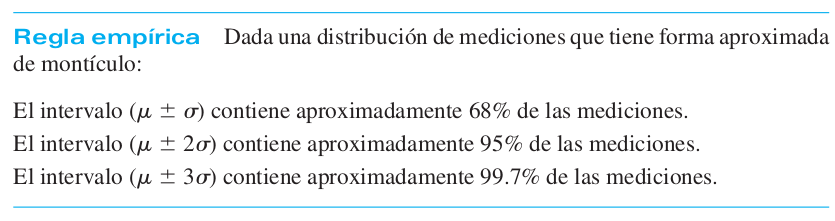
\includegraphics[scale=0.4]{im21}
\end{center}


\end{frame}
%%%%%%%%%%%%%%%%%%%%%%%%%%%%%%%%%%%%%%%%%%%%%%%%%%%%%%%%%%%%%%%%%%%%%%%%%%%%%%%%%%%%%%%%%%%%%%%%%%%%%%%%%%%%%
\begin{frame}
\frametitle{Regla empírica}
Ejercicio 

En un estudio de tiempo efectuado en una planta manufacturera, el tiempo para completar una operación especificada se mide para cada uno de los $n= 40$ trabajadores. Se encuentra que la media y la desviación estándar son 12.8 y 1.7, respectivamente. Describa los datos muestrales usando la Regla empírica.


\end{frame}
%%%%%%%%%%%%%%%%%%%%%%%%%%%%%%%%%%%%%%%%%%%%%%%%%%%%%%%%%%%%%%%%%%%%%%%%%%%%%%%%%%%%%%%%%%%%%%%%%%%%%%%%%%%%%
\begin{frame}
\frametitle{Regla empírica}
\begin{center}
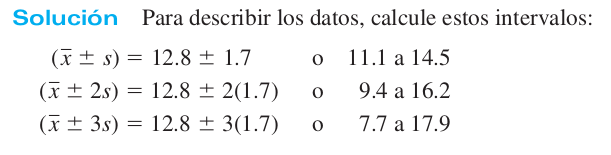
\includegraphics[scale=0.4]{im22}
\end{center}
De acuerdo con la Regla empírica, se espera que aproximadamente 68\% de las mediciones caigan en el intervalo de 11.1 a 14.5, aproximadamente 95\% caigan en el intervalo de 9.4 a 16.2, y aproximadamente 99.7\% caigan en el intervalo de 7.7 a 17.9.

\end{frame}
%%%%%%%%%%%%%%%%%%%%%%%%%%%%%%%%%%%%%%%%%%%%%%%%%%%%%%%%%%%%%%%%%%%%%%%%%%%%%%%%%%%%%%%%%%%%%%%%%%%%%%%%%%%%%
\begin{frame}
\frametitle{Ejercicio}
Los maestros-estudiantes son capacitados para desarrollar planes de lecciones, en la suposición de que el plan escrito les ayudará a trabajar de manera satisfactoria en el salón de clases. En un estudio para evaluar la relación entre planes de lección escritos y su implementación en el salón de clases, se calificaron 25 planes de lección en una escala de 0 a 34 de acuerdo a una Lista de verificación de Plan de lección. Las 25 calificaciones se
muestran en la tabla. Use el teorema de Chebyshev y la Regla empírica (si es aplicable) para describir la distribución de estas calificaciones de evaluación.
\begin{center}
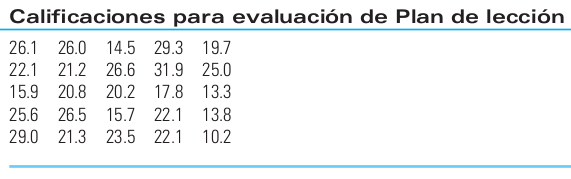
\includegraphics[scale=0.4]{im23}
\end{center}


\end{frame}
%%%%%%%%%%%%%%%%%%%%%%%%%%%%%%%%%%%%%%%%%%%%%%%%%%%%%%%%%%%%%%%%%%%%%%%%%%%%%%%%%%%%%%%%%%%%%%%%%%%%%%%%%%%%%
\begin{frame}
\frametitle{Mediciones de posición relativa }
A veces es necesario conocer la posición de una observación respecto a otras de un conjunto de datos.

\begin{block}{Definición}
El \textbf{puntaje z muestral} es una medida de posición relativa definida
por
\begin{equation*}
\text{puntaje } z = \frac{x-\bar{x}}{s}
\end{equation*}
\end{block}

Un puntaje z mide la distancia entre una observación y la media, medidas en unidades de desviación estándar.

\end{frame}
%%%%%%%%%%%%%%%%%%%%%%%%%%%%%%%%%%%%%%%%%%%%%%%%%%%%%%%%%%%%%%%%%%%%%%%%%%%%%%%%%%%%%%%%%%%%%%%%%%%%%%%%%%%%%
\begin{frame}
\frametitle{Mediciones de posición relativa }
Por ejemplo, suponga que la media y desviación estándar de los puntajes de examen (basados en un total de 35 puntos) son 25 y 4, respectivamente. El puntaje z para una calificación de 30 se calcula como sigue:

\begin{equation*}
\text{puntaje } z = \frac{x-\bar{x}}{s}=\frac{30-25}{4}=1.25
\end{equation*}

El puntaje de 30 está a 1.25 desviaciones estándar arriba de la media $(30 = \bar{x}+1.25s)$.
\end{frame}
%%%%%%%%%%%%%%%%%%%%%%%%%%%%%%%%%%%%%%%%%%%%%%%%%%%%%%%%%%%%%%%%%%%%%%%%%%%%%%%%%%%%%%%%%%%%%%%%%%%%%%%%%%%%%
\begin{frame}
\frametitle{Mediciones de posición relativa }
\begin{center}
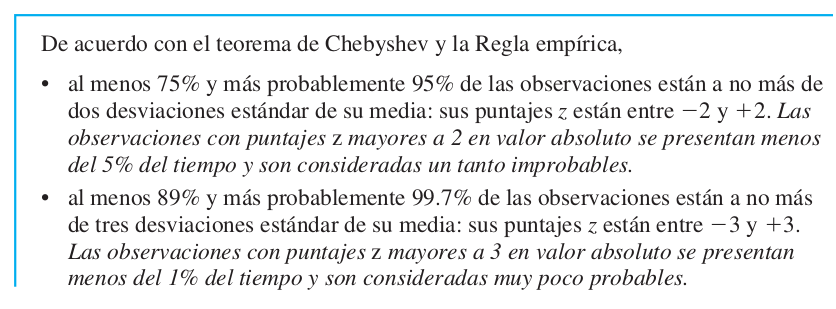
\includegraphics[scale=0.4]{im24}
\end{center}
\end{frame}
%%%%%%%%%%%%%%%%%%%%%%%%%%%%%%%%%%%%%%%%%%%%%%%%%%%%%%%%%%%%%%%%%%%%%%%%%%%%%%%%%%%%%%%%%%%%%%%%%%%%%%%%%%%%%
\begin{frame}
\frametitle{Percentil}
Un percentil es otra medida de posición relativa y se usa con más frecuencia para conjuntos grandes de datos. (Los percentiles no son muy útiles para conjuntos pequeños de datos).

\begin{block}{Definición}
Un conjunto de n mediciones de la variable $x$ se ha reacomodado en
orden de magnitud. El p-ésimo percentil es el valor de $x$ que es mayor a $p\%$ de las mediciones y es menor que el restante $(100 - p)\%$.
\end{block}


\end{frame}
%%%%%%%%%%%%%%%%%%%%%%%%%%%%%%%%%%%%%%%%%%%%%%%%%%%%%%%%%%%%%%%%%%%%%%%%%%%%%%%%%%%%%%%%%%%%%%%%%%%%%%%%%%%%%
\begin{frame}
\frametitle{Percentil}
Supongamos que usted ha sido notificado que su calificación de 610, en el Examen verbal de graduación, lo ha colocado en el 60avo percentil en la distribución de calificaciones. ¿Dónde está su calificación de 610 en relación a las calificaciones de los otros que tomaron el examen?

\vspace{1em}
Solución Calificar en el 60avo percentil significa que $60\%$ de todas las calificaciones de examen fueron más bajas que la calificación de usted y $40\%$ fueron más altas.

\end{frame}
%%%%%%%%%%%%%%%%%%%%%%%%%%%%%%%%%%%%%%%%%%%%%%%%%%%%%%%%%%%%%%%%%%%%%%%%%%%%%%%%%%%%%%%%%%%%%%%%%%%%%%%%%%%%%
\begin{frame}
\frametitle{Percentil}
En general, el 60avo percentil para la variable x es un punto en el eje horizontal de la distribución de datos que es mayor a 60\% de las mediciones y menor que las otras.

\begin{center}
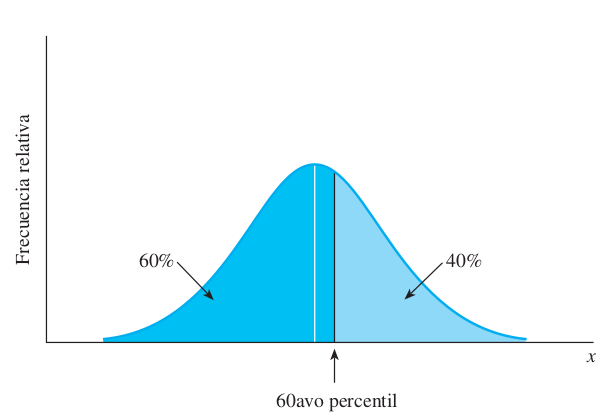
\includegraphics[scale=0.4]{im25}
\end{center}

\end{frame}
%%%%%%%%%%%%%%%%%%%%%%%%%%%%%%%%%%%%%%%%%%%%%%%%%%%%%%%%%%%%%%%%%%%%%%%%%%%%%%%%%%%%%%%%%%%%%%%%%%%%%%%%%%%%%
\begin{frame}
\frametitle{Percentil-Cuartil}

\begin{itemize}
\item La mediana es igual que el 50avo percentil.
\item Los percentiles 25avo y 75avo, llamados cuartiles inferior y superior
\item Veinticinco por ciento de las mediciones serán menores que el cuartil inferior (primero).
\item 50\% serán menores que la mediana (el segundo cuartil).
\item 75\% serán menores que el cuartil superior (tercero).
\end{itemize}

\end{frame}
%%%%%%%%%%%%%%%%%%%%%%%%%%%%%%%%%%%%%%%%%%%%%%%%%%%%%%%%%%%%%%%%%%%%%%%%%%%%%%%%%%%%%%%%%%%%%%%%%%%%%%%%%%%%%
\begin{frame}
\frametitle{Cuartil}

\begin{center}
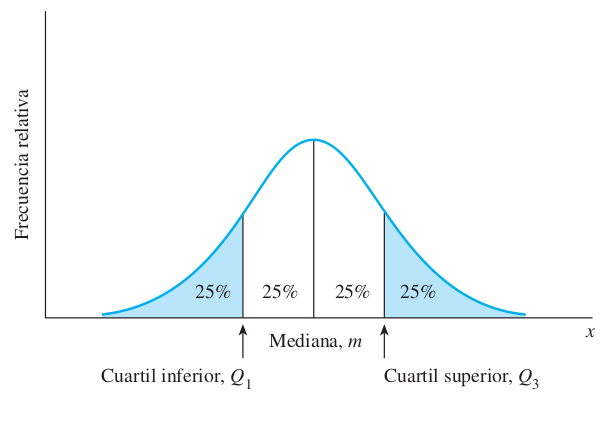
\includegraphics[scale=0.4]{im26}
\end{center}

\end{frame}
%%%%%%%%%%%%%%%%%%%%%%%%%%%%%%%%%%%%%%%%%%%%%%%%%%%%%%%%%%%%%%%%%%%%%%%%%%%%%%%%%%%%%%%%%%%%%%%%%%%%%%%%%%%%%
\begin{frame}
\frametitle{Cuartil}

\begin{block}{Definición}
Un conjunto de $n$ mediciones en la variable $x$ se ha acomodado en orden
de magnitud. El \textbf{cuartil inferior (primer cuartil), $Q_{1}$ }, es el valor de $x$ que es mayor a un cuarto de las mediciones y es menor que los restantes tres cuartos. El s\textbf{egundo cuartil} es la mediana. El \textbf{cuartil superior (tercer cuartil), $Q_{3}$ }, es el valor de $x$ que es mayor a tres cuartos de las mediciones y es menor que el restante un cuarto.
\end{block}

\end{frame}
%%%%%%%%%%%%%%%%%%%%%%%%%%%%%%%%%%%%%%%%%%%%%%%%%%%%%%%%%%%%%%%%%%%%%%%%%%%%%%%%%%%%%%%%%%%%%%%%%%%%%%%%%%%%%
\begin{frame}
\frametitle{Cuartil}

\begin{center}
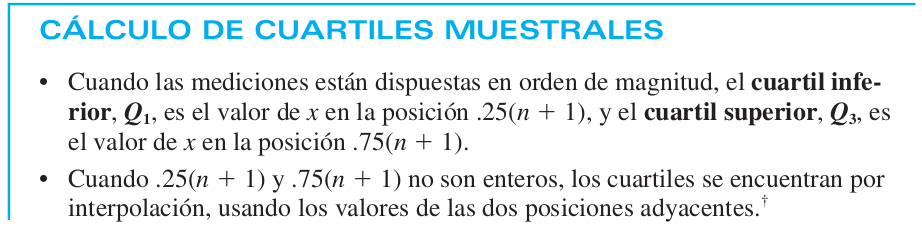
\includegraphics[width=\textwidth]{im27}
\end{center}


\end{frame}
%%%%%%%%%%%%%%%%%%%%%%%%%%%%%%%%%%%%%%%%%%%%%%%%%%%%%%%%%%%%%%%%%%%%%%%%%%%%%%%%%%%%%%%%%%%%%%%%%%%%%%%%%%%%%
\begin{frame}
\frametitle{Cuartil}

\begin{center}
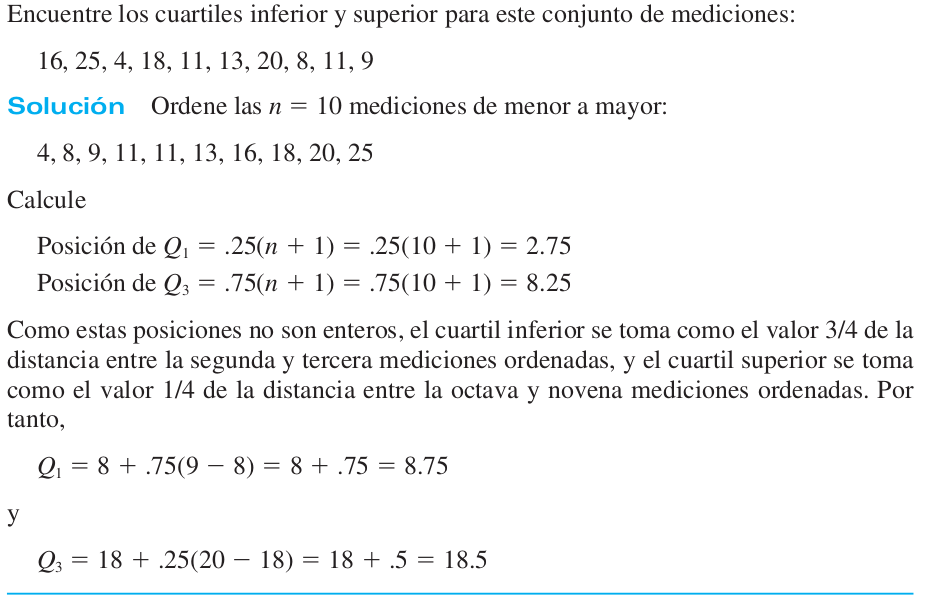
\includegraphics[width=\textwidth]{im28}
\end{center}


\end{frame}
%%%%%%%%%%%%%%%%%%%%%%%%%%%%%%%%%%%%%%%%%%%%%%%%%%%%%%%%%%%%%%%%%%%%%%%%%%%%%%%%%%%%%%%%%%%%%%%%%%%%%%%%%%%%%
\begin{frame}
\frametitle{Intercuartil}
Como la mediana y los cuartiles dividen la distribución de datos en cuatro partes, cada una de ellas conteniendo alrededor de 25\% de las mediciones, $Q_1$ y $Q_3$ son las fronteras superior e inferior para el 50\% central de la distribución. Podemos medir el rango de este “50\% central” de la distribución usando una medida numérica llamada rango intercuartil.

\begin{block}{Definición}
El rango intercuartil (IQR) para un conjunto de mediciones es la diferencia entre los cuartiles superior e inferior; esto es, $IQR = Q_3 - Q_1$ .
\end{block}
\end{frame}
%%%%%%%%%%%%%%%%%%%%%%%%%%%%%%%%%%%%%%%%%%%%%%%%%%%%%%%%%%%%%%%%%%%%%%%%%%%%%%%%%%%%%%%%%%%%%%%%%%%%%%%%%%%%%
\begin{frame}
\frametitle{El resumen de cinco números y la gráfica de caja}


\begin{center}
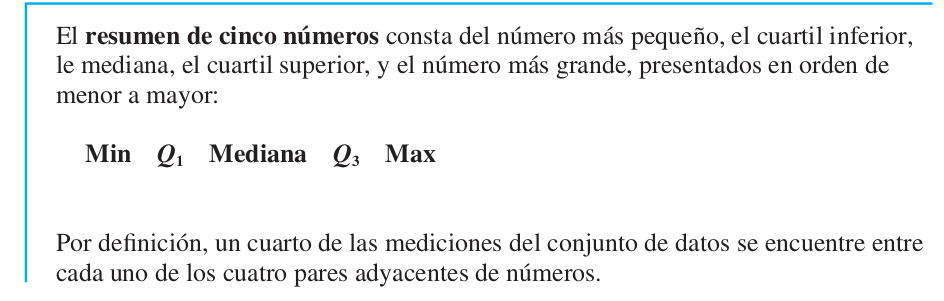
\includegraphics[width=\textwidth]{im29}
\end{center}

\end{frame}
%%%%%%%%%%%%%%%%%%%%%%%%%%%%%%%%%%%%%%%%%%%%%%%%%%%%%%%%%%%%%%%%%%%%%%%%%%%%%%%%%%%%%%%%%%%%%%%%%%%%%%%%%%%%%
\begin{frame}
\frametitle{El resumen de cinco números y la gráfica de caja}


\begin{center}
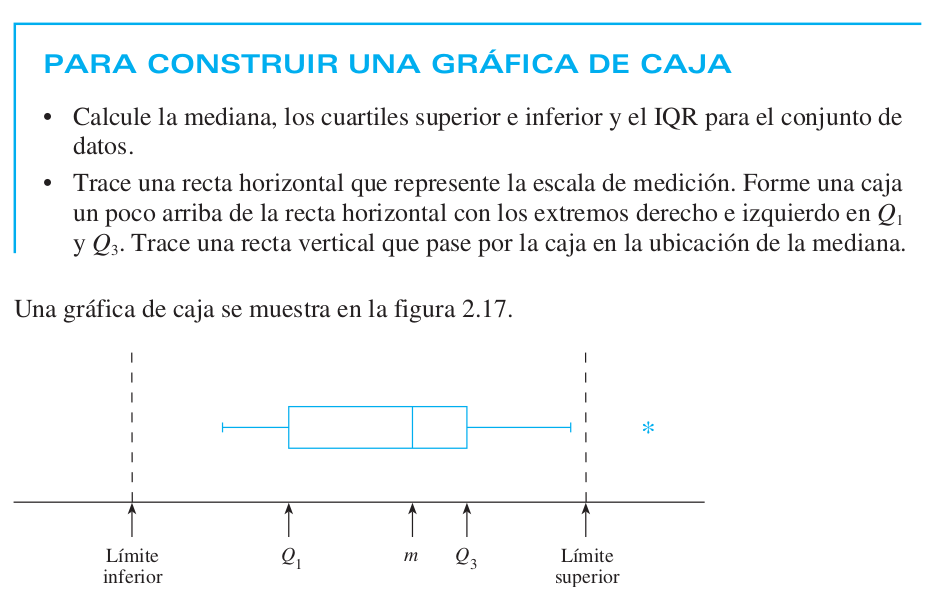
\includegraphics[width=\textwidth]{im30}
\end{center}

\end{frame}
%%%%%%%%%%%%%%%%%%%%%%%%%%%%%%%%%%%%%%%%%%%%%%%%%%%%%%%%%%%%%%%%%%%%%%%%%%%%%%%%%%%%%%%%%%%%%%%%%%%%%%%%%%%%%
\end {document}



                                                  






